% roba — dual-arm robotic meat-cutting simulation (Aim 3.3)
% Build: pdflatex main && pdflatex main   (no bibtex needed — refs are inline)
\documentclass[conference]{IEEEtran}
\usepackage{graphicx,amsmath,booktabs,hyperref,url,xcolor}
\graphicspath{{../experiments/out/}}

\title{roba: A Dual-Arm Robotic Meat-Cutting Simulation in NVIDIA Isaac Sim with\\
Layered Breakable-Seam Cutting, IK-Driven Manipulation, and a Video-Grounded Control Study}
\author{\IEEEauthorblockN{T. Tang}\IEEEauthorblockA{Boston University \\ tztang@bu.edu}}

\begin{document}
\maketitle

\begin{abstract}
We present \emph{roba}, an open dual-arm robotic meat-cutting simulation built on NVIDIA Isaac Sim,
together with a data-driven control and modeling study aimed at meat cutting with an eye toward
surgical extension. The central technical obstacle is that Isaac Sim / PhysX cannot topologically cut
a deformable continuum at runtime; we verify this limitation and resolve it with a \emph{layered
breakable-seam} model in which a three-layer pork-belly slab (skin, fat, lean) is authored as rigid
sub-blocks joined by breakable fixed joints whose break forces are derived from each tissue's fracture
toughness. We show in PhysX that (i) the simulator dynamically honors these per-layer break forces
($<2.5\%$ error for fat and skin; the ordering skin $\gg$ fat $>$ lean is reproduced), (ii) a
constant-depth tangential pass selectively peels the skin layer (a novel sub-task), and (iii) a 7-DOF
arm under Jacobian inverse kinematics descends a knife through the slab as a robot-driven cut. We
further survey the control theory of food and surgical cutting, run a video-to-trajectory perception
pipeline that recovers a kinematic cutting model from footage, and document that quantitative
\emph{forces} are not recoverable from RGB and must come from sensors/simulation. All physics results
were produced headless; we contribute a driver-agnostic recorder/renderer that visualizes the cut
without the GPU's ray-tracing path. We release code, experiments, and figures.
\end{abstract}

\section{Introduction}
\label{sec:intro}
Robotic cutting of soft, layered biological material is a contact-rich, fracture-driven manipulation
problem with applications from food processing to surgery. We target meat cutting (pork belly) as the
primary use case, with the longer-term goal of transferring methods toward surgical cutting and
resection. We build on NVIDIA Isaac Sim as the simulation platform and integrate open robot arms
(OpenArm by Enactic; reBot~B601 by Seeed).

Our contributions are:
\begin{itemize}
  \item An open, reproducible dual-arm cutting simulation with a three-layer pork-belly material model.
  \item A \emph{layered breakable-seam} cutting model that works within Isaac Sim / PhysX despite the
        absence of native deformable cutting, with break forces grounded in tissue fracture mechanics.
  \item PhysX validation that the simulator honors the per-layer break-force model and reproduces the
        skin~$\gg$~fat~$>$~lean cutting-resistance ordering.
  \item A first demonstration of \emph{constant-depth skin skiving} as a selective-peel sub-task, and a
        vertical-slicing sub-task, both validated in simulation.
  \item An IK-driven dual-arm cut (one arm holds via impedance, the other cuts) and a two-variable
        plane-constrained control interface.
  \item A decoupled video-understanding pipeline that recovers a kinematic cutting trajectory from
        footage, with an explicit account of why forces are not recoverable from RGB alone.
  \item A driver-agnostic recording/replay renderer that sidesteps a GPU-driver limitation on our
        cluster.
\end{itemize}

\section{Related Work}
\label{sec:related}
Food-cutting research has established the mechanics of knife motion, notably the \emph{slice-push}
(pressing--slicing) ratio that quantifies how lateral blade motion reduces the normal force required to
fracture material (Jia and colleagues), and differentiable cutting simulation (DiSECt) for parameter
inference and control. Surgical autonomy has advanced from supervised-autonomy suturing to the
hierarchical, language-conditioned imitation framework SRT-H, which autonomously performed the
clip-and-cut phase of cholecystectomy on \emph{ex-vivo} tissue. Across both domains, force/hybrid
position--force control governs contact, impedance/admittance control provides compliance, and visual
servoing guides cut geometry; mature systems layer these rather than relying on any one. We draw on
this literature (see the project's \texttt{CONTROL\_SURVEY.md} and \texttt{REFERENCES.md} for the full
set of $\sim$150 sources) and adopt the slice-push mechanics and a hierarchical control posture.

\section{Background: The Cutting-Simulation Problem}
\label{sec:bg}
We verified that Isaac Sim / PhysX~5 cannot cut a deformable soft body at runtime: FEM soft bodies use
a fixed tetrahedral mesh, no API exposes tearing/re-tetrahedralization, and NVIDIA staff state cutting
is unsupported. Popular ``cutting in Isaac Sim'' demonstrations are breakable-joint approximations of
pre-segmented geometry. Genuine topological cutting is solved outside core PhysX (FEM element deletion,
XFEM, or the Material Point Method). We therefore adopt two representations: a \emph{breakable-seam}
model for in-engine, real-time cutting (this paper), and DiSECt/MPM as a physics-faithful path for
force calibration (future work). Table~\ref{tab:design} summarizes the design space.

\begin{table}[t]\centering\small
\caption{Cutting-representation design space.}\label{tab:design}
\begin{tabular}{@{}lll@{}}\toprule
Option & Pro & Con \\ \midrule
Breakable seams (ours) & real-time, in-engine & cuts follow pre-scored seams \\
DiSECt (diff. FEM) & force-faithful, calibratable & separate engine \\
MPM & natural severing & integration/fidelity cost \\
In-PhysX re-tet & in-engine & no API; research-grade \\ \bottomrule
\end{tabular}
\end{table}

\section{System and Methods}
\label{sec:system}
\subsection{Platform and Arms}
We run Isaac Sim~6.0 (PhysX backend). We load the OpenArm unimanual/bimanual USD (7-DOF per arm,
confirmed by articulation introspection) and import the reBot~B601 URDF. A rigid blade is fixed to the
cutting arm's tool-center-point frame.

\subsection{Three-Layer Breakable-Seam Tissue Model}
The pork belly is a $20\times3$ grid of rigid sub-blocks (skin/fat/lean) joined by breakable fixed
joints. Each seam's break force follows an energy-based form,
$F_{\text{break}} \approx J_c\,w\,(1-0.4\,r)\,s(\rho) + \mu N$,
where $J_c$ is the layer fracture toughness, $w$ the seam width, $r$ the slice-push ratio (a draw cut
lowers force by up to $40\%$), $s(\rho)$ a bounded blade-sharpness factor, and $\mu N$ a friction term.
Toughness priors (skin $\sim$17--30, fat $\sim$4.1, lean $\sim$0.1--0.8~kJ/m\textsuperscript{2}) come
from the literature; absolute values require local calibration.

\subsection{Dual-Arm Control}
The holding arm is set to compliant (low-stiffness/damping) joint gains and welds the workpiece to its
gripper once positioned (impedance hold). The cutting arm uses a finite-difference-Jacobian
damped-least-squares position IK: we perturb each joint, measure the end-effector displacement by
forward kinematics, and solve $\Delta q = J^\top (JJ^\top + \lambda^2 I)^{-1} e$. Because the home pose
sits at the bottom of the workspace, a cut is executed as raise-then-descend.

\subsection{Two-Variable Plane-Constrained Interface}
The cutting task is reduced to a vertical plane: end-effector orientation and the out-of-plane axis are
fixed, and two control variables map to in-plane $(x,z)$. A normalized 2-D signal (a mouse cursor, or a
recorded/extracted path) drives these two variables through the IK, so only two of six task-space DOF
are commanded. (Live mouse input requires the GUI; we exercise the interface with recorded paths.)

\subsection{Driver-Agnostic Visualization}
On our cluster the GPU driver blocks Isaac's RTX renderer, but headless physics runs. We record each
box's world pose per frame and replay the geometry with a matplotlib renderer, producing cut videos and
figures with no dependence on the ray-tracing path.

\section{Experiments and Results}
\label{sec:exp}
All results are headless PhysX runs; figures are produced by the driver-agnostic renderer.

\paragraph{Force model (Fig.~\ref{fig:force}).} A ramping pull severs a held block per layer; the
measured break force matches the configured model to $2.3\%$ (fat) and $0.5\%$ (skin), and the ordering
skin~$\gg$~fat~$>$~lean holds (skin requires $\sim$27$\times$ the lean force).

\paragraph{Vertical slicing.} A blade swept down at three stations produces a monotonic cut
progression, breaking in-layer and inter-layer seams as it crosses each layer.

\paragraph{Skin skiving (Fig.~\ref{fig:skive}).} A constant-depth tangential pass severs $20/20$
skin/fat interfaces (peel fraction $1.0$) while leaving the lean/fat interface and the in-skin seams
intact---a selective peel that lifts the skin as a connected sheet.

\paragraph{IK-driven dual-arm cut (Fig.~\ref{fig:ik}).} The cutting arm raises to a clear pose and
descends the knife through the slab; seams break precisely as the blade crosses the layers.

\paragraph{Video to trajectory (Fig.~\ref{fig:traj}).} The perception pipeline recovers the knife's
press-push-slice path and phase structure from video (mean normalized tracking error $0.16$; the bias
reflects centroid-vs-tip tracking). Forces are not recovered from RGB by design.

\begin{figure}[t]\centering
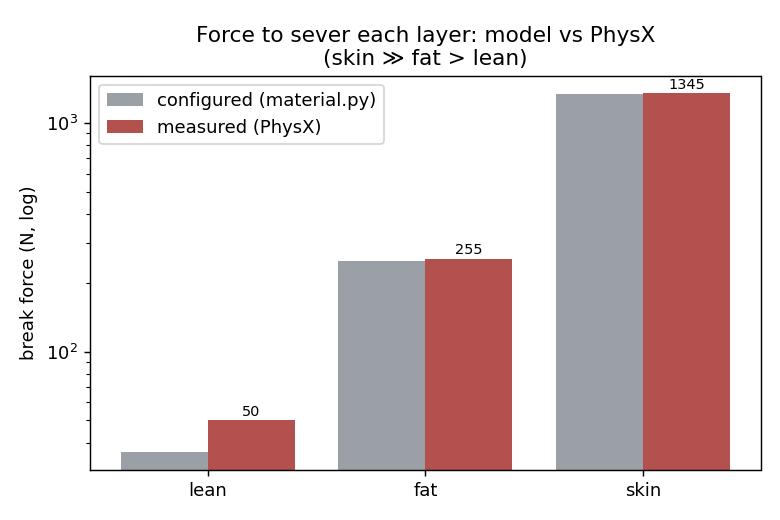
\includegraphics[width=0.82\linewidth]{force_break.png}
\caption{Configured vs.\ PhysX-measured break force per layer (log scale).}\label{fig:force}
\end{figure}
\begin{figure}[t]\centering
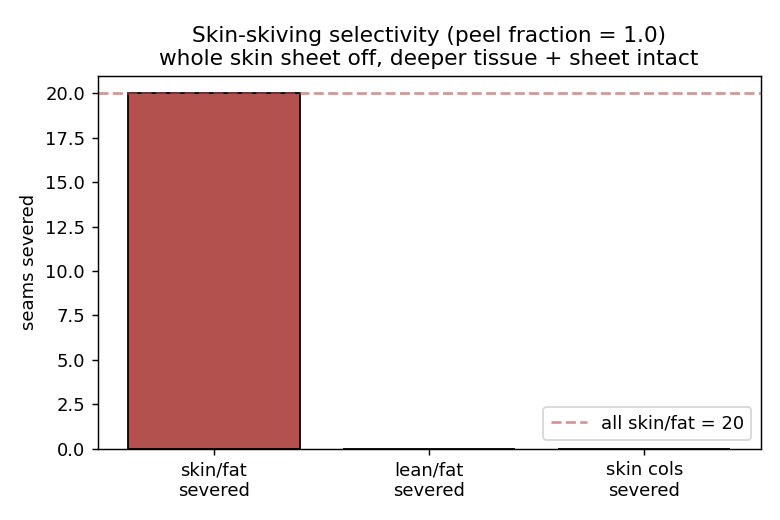
\includegraphics[width=0.82\linewidth]{skive_selectivity.png}
\caption{Skin-skiving selectivity: only the skin/fat interface is severed.}\label{fig:skive}
\end{figure}
\begin{figure}[t]\centering
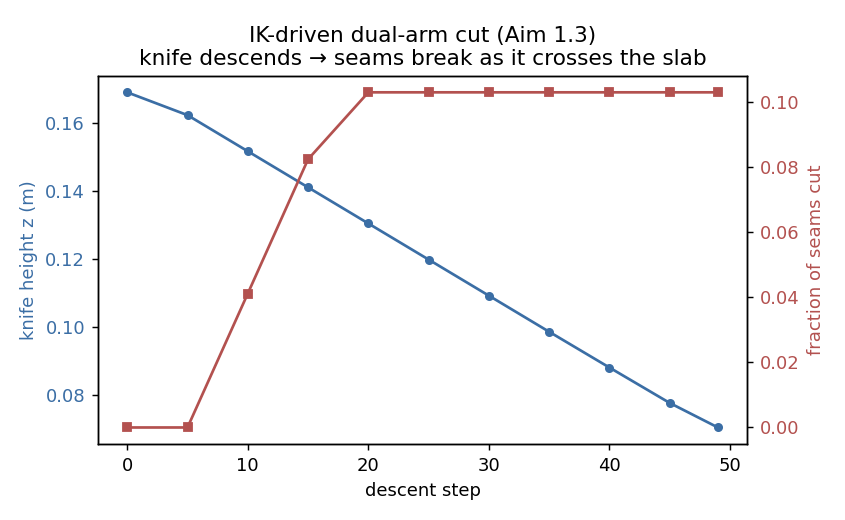
\includegraphics[width=0.82\linewidth]{ik_cut.png}
\caption{IK-driven cut: knife descent (blue) vs.\ cut fraction (red).}\label{fig:ik}
\end{figure}
\begin{figure}[t]\centering
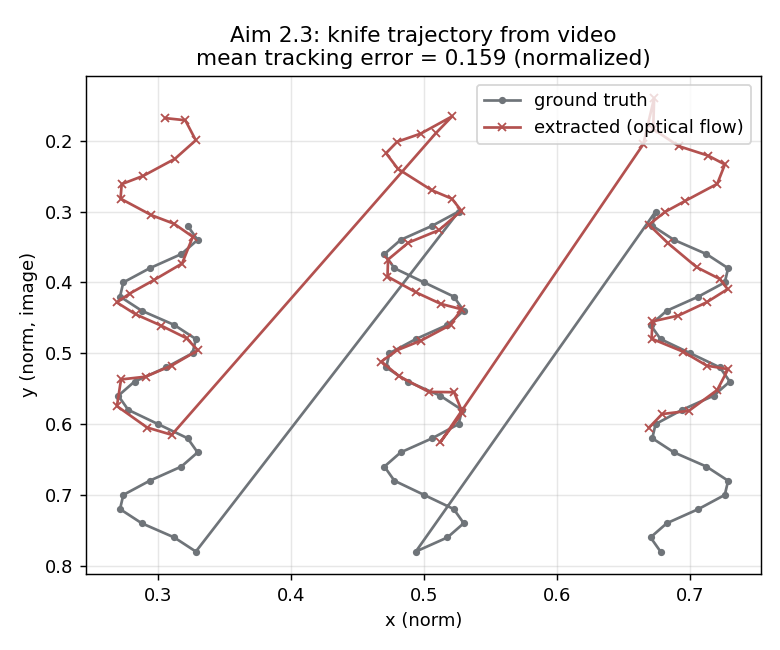
\includegraphics[width=0.82\linewidth]{traj_validation.png}
\caption{Knife trajectory recovered from video vs.\ ground truth.}\label{fig:traj}
\end{figure}

\section{Limitations}
\label{sec:limits}
(1) Breakable seams cut along predetermined lines, not arbitrary continuum paths; true severing needs
DiSECt/MPM. (2) Cutting forces are not recoverable from RGB video; our force model is simulation-only
until a force/torque sensor is integrated. (3) Material parameters carry order-of-magnitude
uncertainty and muscle anisotropy; local calibration is required. (4) Results are simulation-only with
no hardware sim-to-real. (5) Live mouse/GUI interaction and RTX rendering are blocked by a cluster GPU
driver regression; we visualize via the driver-agnostic renderer instead. (6) Skin skiving is validated
in simulation only; no real-tissue closed-loop baseline exists.

\section{Conclusion}
\label{sec:conclusion}
roba demonstrates a reproducible dual-arm meat-cutting simulation whose layered breakable-seam model is
grounded in tissue fracture mechanics and validated in PhysX, alongside a video-grounded control study.
Future work: DiSECt/MPM force-faithful cutting, a hierarchical learned controller in the SRT-H mold,
real force-sensor calibration, and sim-to-real transfer.

\section*{Reproducibility}
Code, pinned environment, the SCC run kit, experiment results, and all figures are released in the
project repository. NVIDIA assets are not redistributed; a setup script fetches them.

\end{document}
